%%%%%%%%%%%%%%%%%%%%%%%%%% author.tex %%%%%%%%%%%%%%%%%%%%%%%%%
%
% sample root file for your contribution to an IFIP volume
% published at Springer
%
% Use this file as a template for your own input.
%
%%%%%%%%%%%%%%%%%%%%%%%% Springer-Verlag %%%%%%%%%%%%%%%%%%%%%%%%%%


% RECOMMENDED %%%%%%%%%%%%%%%%%%%%%%%%%%%%%%%%%%%%%%%%%%%%%%%%%%%
\documentclass[ifip]{svmult}

% choose options for [] as required from the list
% in the Reference Guide, Sect. 2.2
\usepackage{url}
\usepackage{epsfig}
\usepackage{makeidx}         % allows index generation
\usepackage{graphicx}        % standard LaTeX graphics tool
                             % when including figure files
\usepackage{multicol}        % used for the two-column index
\usepackage[bottom]{footmisc}% places footnotes at page bottom
\usepackage{float}           % H para posicionar figuras
\usepackage{booktabs}
% etc.
% see the list of further useful packages
% in the Reference Guide, Sects. 2.3, 3.1-3.3

\makeindex             % used for the subject index
                       % please use the style sprmidx.sty with
                       % your makeindex program


%%%%%%%%%%%%%%%%%%%%%%%%%%%%%%%%%%%%%%%%%%%%%%%%%%%%%%%%%%%%%%%%%%%%%

\begin{document}

\title*{BugTracking: A tool to assist in the identification of bug reports}
% Use \titlerunning{Short Title} for an abbreviated version of
% your contribution title if the original one is too long
\author{Gema Rodriguez\inst{1}, Jesus M. Gonzalez-Barahona\inst{1} \and Gregorio Robles\inst{1}}
%\and Name of Author\inst{2}}
% Use \authorrunning{Short Title} for an abbreviated version of
% your contribution title if the original one is too long
\institute{\texttt{gerope@libresoft.es},\texttt{jgb@gsyc.es},\texttt{grex@gsyc.es}
\and GSyC/LibreSoft, Universidad Rey Juan Carlos}
%
% Use the package "url.sty" to avoid
% problems with special characters
% used in your e-mail or web address
%
\maketitle

\begin{abstract}
	In most software projects, but in particular in almost all free, open source software projects, issue tracking systems are used for recording many different kinds of issues: bug reports, feature requests, maintenance tickets, and even design discussions. Identifying which of those issues are bug reports, is not a trivial task. When researchers want to conduct some study on the bug reports managed by a software development project, they need to first of all to perform this identification.\\

The job for researchers here is very different from the bug triaging that developers do. In the latter case, people with a lot of experience in the project make a decision based on the information available at that time (maybe just a short comment by some user), asking if needed for more details. In the former case, researchers are usually not that experienced in the project, but they have at their disposal all the information produced, until the moment the issue was closed. This may include not only all comments and actions on the issue tracking system, but for examples, discussions about a fix in the code review system, or the final fixing patch in the source code management system. Having all that information conveyed to the researchers in an easy, flexible and quick way accelerates and makes much more reliable their decision making process. This simplifies large scale manual analysis of issues (in the hundreds or thousands), helping researchers to ensure that they are really working with what they intend to work: bug reports.\\

This paper presents a tool designed exactly to solve this problem of providing the researcher with all the relevant information needed to decide if an issue corresponds to a bug report or not. The tool uses information extracted automatically from the project repositories, and offers a web-based interface which allows for collaboration, traceability and transparency of the identification of bug reports, making the process easier, faster, and more reliable.
\end{abstract}

\section{Introduction}
\label{sec:1}

%Many efforts on how and why bugs are introduced in the software source code are underway in the software engineering research community. Software source code is affected by many changes, many of them due to failure of the software because of emergent bugs.

While a software system is being developed, software engineers use version repositories to produce and manage their code. Developers and tester report issues, which are stored in other repositories, known as issue-tracking system, where many kinds of issues can be found.

Issue-tracking systems help solving these bugs, but their problem is the difficulty of distinguish the bug reports from other that are not bugs. These systems provide an interface to manage reports of maintenance activities where developers can report issues describing bug reports, features or code optimizations. During the bug triage process it is difficult to distinguish bug reports from other issues; a study describes that two of five issues are misclassified~\cite{Herzig}. This misclassification causes bias predicting bugs where non-bug reports are taken into account.

To distinguish the bug reports we can use automatic classification systems as the one described in~\cite{Antoniol}, but the vocabulary used in the issues could change from project to project, as well as the policy depending on the project. Consequently, data validation is recommended in the studies~\cite{Herzig}.

Linking a bug reports in a issue-tracking system and the corresponding fix-commit may be not a trivial task. Traditionally, the methods used in link recovery~\cite{Zimmermann, Thomas} are based on text patterns or the mining of key phrases. Unfortunately, these methods can include many false negatives causing bias in data~\cite{Bird, NguyenTH}. Therefore other methods, such as Mlink approach, have been developed to link bug report with fixes using features in the changed source files corresponding to commit logs in addition to the traditional textual features~\cite{Nguyen}. But all of them suppose that the issues are bug reports.

In this paper, we present a tool to display all the data necessary to the developers who will decide whether the issue is a bug report or not. The developers have the best available knowledge of their system, therefore the tool will help them choosing only bug reports, removing any bias induced by non bug reports.


\section{The tool}
\label{sec:2}

The tool works in the browser, displaying the main characteristics to distinguish bug report from others. Developers will be responsible to classify the tickets as bug report or not, could explain their decisions in each ticket.


\subsection{Architecture}

This tool works with Launchpad as issue-tracking system and Gerrit as code review system. The image \ref{fig:1} presents the architecture used, which has been developed with JavaScript, Node, JQuery and HTML5 technologies. The server side works making queries to the API of Gerrit an Launchpad, and the client side is where the user can see the information displayed, and interacts with the server through events. Both sides share the information required using JSON files and use their own REST API. Furthermore, to integrate some functionalities from GitHub, we use a third-party application between GitHub and the browser.

\label{sec:2.1}
\begin{figure}
\centering
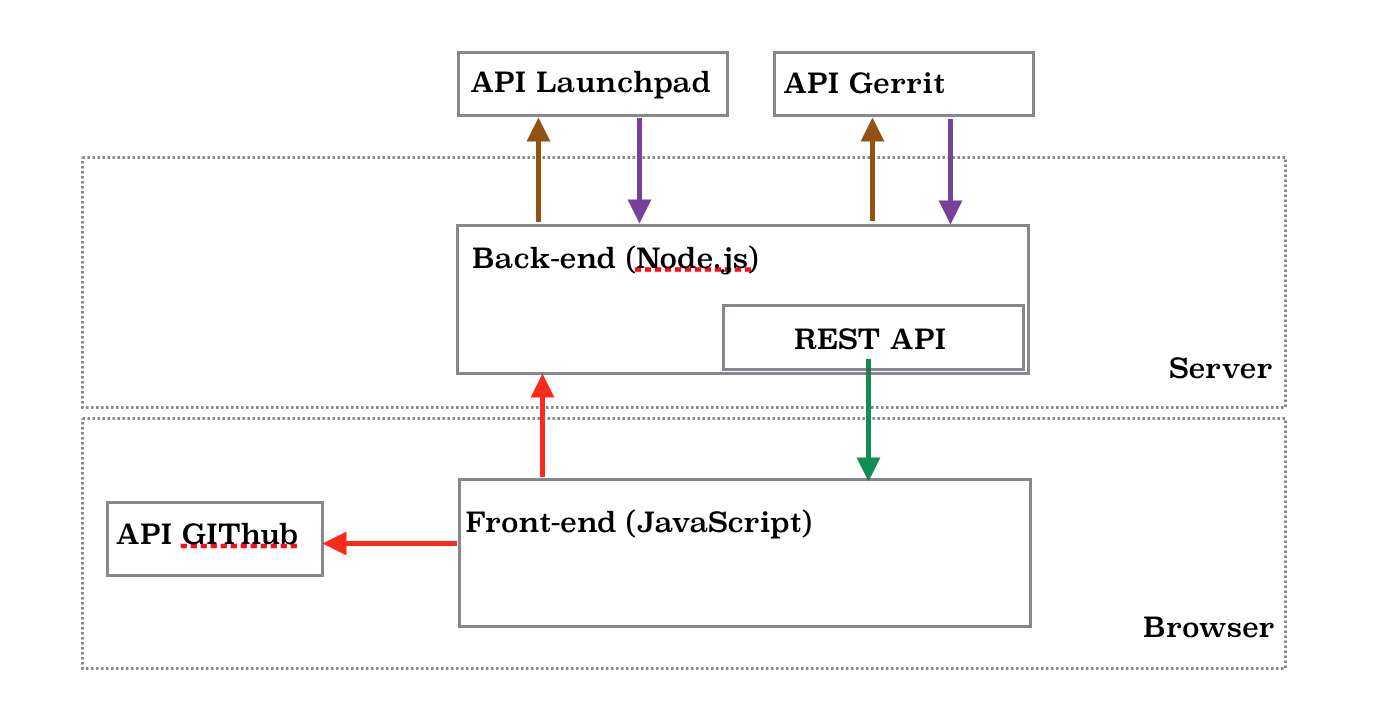
\includegraphics[height=7cm]{Arquitectura.png}
\caption{Architecture of the tool.}
\label{fig:1}       % Give a unique label
\end{figure}

\subsection{Main Features}
\label{sec:2.2}
The tool shows the id of the tickets, which are extracted randomly from each issue-tracking repository of OpenStack, and displays the information necessary to decide whether the issue is a bug report or not. We focused in display the main parameters that help in the classification, such as the title of the report and the description as well as the description of the fix commit.

The left side in the image \ref{fig:2}, shows the information related with the ticket in Launchpad and its correspondent review in Gerrit. Some information displayed link with the original web pages in Launchpad and Gerrit, thereby the developers have at their disposal extra information such as the comments that other developers have done. Could tracking the history since the ticket opens until the commit fixed the ticket.

The right side is guided to user's opinion, after reading all the information displayed, they have to classify the ticket as \textit{Bug report} or \textit{Not Bug report}. Due to unsophisticated description used in the ticket, the developers could doubt in the classification, for this reason we add an extra option in the classification, \textit{Undecided}. Furthermore, the developers have a textarea to write their opinion about their classification in each ticket, as well as other textareas to write the keywords found in the title and the description which can help us building an automatic classification system in the future.

The tool allow carry out a double bind analysis, due to the data is saved in a file in GitHub user's account. GitHub is a control version system in which we have access to the whole information of each commit submitted by the developer. Thus, saving the data in GitHub, we could measure the time that each developer spend in the analysis, which tickets were more difficult to analyze and other statistics that can help us understanding the current problem of issues misclassification.

\begin{figure}
\centering
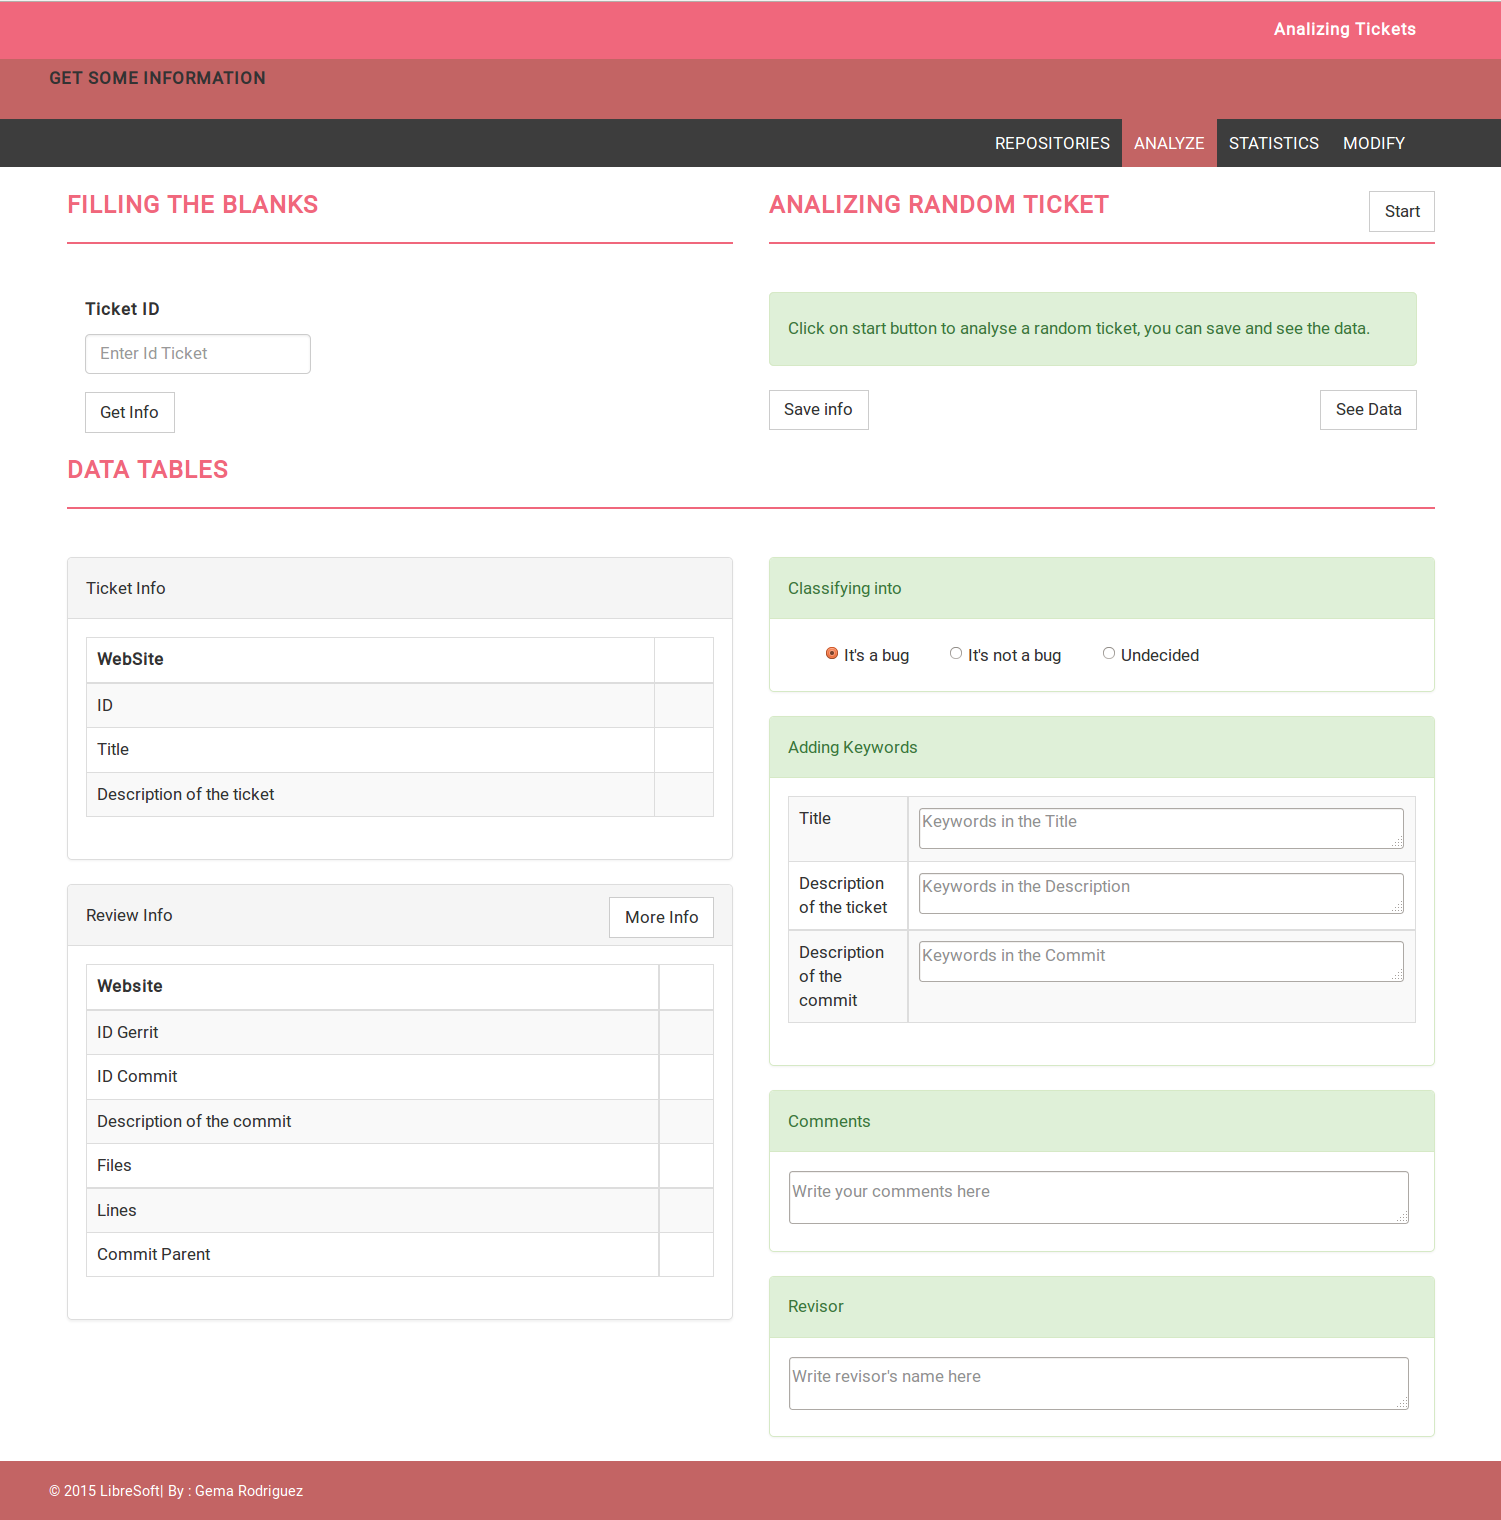
\includegraphics[height=15cm]{index2.png}
\caption{Screenshot of Analyze Tab}
\label{fig:2}       % Give a unique label
\end{figure}

The web page provide us different functionalities depend on in which tab we are, next we explain these functionalities.
\begin{enumerate}
  \item Tab Repository: In this tab we choose which repository of OpenStack we want analyze. Currently the tool supports the four principal repositories: Cinder, Nova, Neutron and Horizon, in which there is more activity.
  \item Tab Analyze: Is the Tab showed in \ref{fig:2} where the user select/insert an identifier of a ticket and analyze with all the data displayed if the ticket are a bug report or not.
  \item Tab Statistics: This tab collects the data saved in the user's repository in GitHub after analyze each ticket, and displays a table with the number of tickets classified as \textit{Bug Report},\textit{Not Bug Report} and \textit{Undecided} in the repository and from each developer involved in the analysis, which name has to be selected previously.
  \item Tab Modify: In this tab, the user can see all his data saved in the GitHub repository and modify the content of the file that he wants, in case of have inserted a mistake during the analysis.
\end{enumerate}

We continue developing the tool but an initial version is available\footnote{\url{bugtracking.libresoft.es}}, as well as a demonstration video\footnote{\url{https://www.youtube.com/watch?v=q0-TIvL4mqc&feature=youtu.be}}. It presents a license type GPL 0 (General Public License) and you can find the code in my GitHub account\footnote{\url{https://github.com/Gemarodri/BugTracking}}. Anyone can use it regardless of have GitHub account or not. But, the ones with GitHub account are the only ones that can save and modify their data, in addition, one of the requirements to save and modify data is create a new repository with the same name that the repository of OpenStack which you want to analyze.

%\section{Validation Study}
%\label{sec:3}

%OpenStack was particularly of interest because of its highest scope and heterogeneous nature with hundreds of developers contributing, furthermore due to its short life, only 5 years, all history is saved and available in a version control system. The issues are called tickets in OpenStack and available in the Launchpad, a web interface of ticket tracking system, classifying them as bug report or not.

%We use the tool to analyze 500 randomly tickets from the four principal repositories in OpenStack. This tickets could be tagged as either "Fix Commited" or "Fix Released", to be able to localize the patch implemented into de source code in the version repository. They are generally tracked in Launchpad \texttt{Nova},\texttt{Cinder},\texttt{Horizon} and \texttt{Neutron}\footnote{\url{https://bugs.launchpad.net/NameOfRepository}}

%The parameters analyzed for each ticket were the title and the description of the report and the description of the fix commit. Also, the code changes if neither the descriptions and the comments clarified the underlying ticket. Each ticket was then categorized into one of three following groups.
%\begin{enumerate}
%  \item The ticket describes a bug report.
%  \item The ticket describes a feature, an optimization code, changes in test files or other not bug reports.
%  \item The ticket presents a vague description and cannot be classified without doubts.
%\end{enumerate}

%Henceforth, we will refer to Group 1 as \textit{Bug Report}, Group 2 as \textit{not Bug Report} and Group 3 as \textit{Undecided}.

%To validate the tool three different developers analyzed tickets belongs to the four main repositories. The developers analyzed more than four hundred tickets to can probe than the tool work as them expected, classifying the tickets into one of the three groups and corroborating that the issues reports present misclassification as ~\cite{Herzig} mentioned.

%In the analysis, some of the tickets present a double bind review process, obtaining that each tickets was analyzed by two developers. %Each developer analyzed 167 tickets plus the half tickets of his teammates. %Only at the end, they discussed the classification conflicts to reach an agreement.

\section{Results}
\label{sec:4}

We have manually analyzed 459 different tickets with support of the present tool, 125 from Cinder, 125 from Nova, 125 from Horizon and 84 from Neutron. The table ~\ref{tab:1} show the percentage of each developer after analyzing the tickets, 417 tickets were analyzed by two different developers, 
\begin{table}[htb]
\begin{center} {\footnotesize
\caption{ Classification statistics of each developer}
\label{tab:1}
\begin{tabular}{lllll}
\toprule[0.3mm]%{\smallskip}
  & Bug Report\kern 1pc & Not Bug Report\kern 1pc & Undecided\kern 1pc & Total \\\hline
Developer 1 \kern 1pc & (184) 55\% & (115) 34\% & (35) 11\% & 334 \\
Developer 2 \kern 1pc & (188) 76\% & (54) 22 \% & (7) 3\% & 249 \\
Developer 3 \kern 1pc & (188) 56\% & (116) 35\% & (30) 9\% & 334 \\
\bottomrule[0.3mm]
\end{tabular} }
\end{center}
\end{table}

The percentages between Developer 1 and Developer 3 are really similar, whereas the Developer 2 has identified more Bug Reports in his analysis. But, the three results support the misclassification present in bug tracking systems. Furthermore, according to ~\cite{Herzig}'s work, approximately two of five issues are misclassified in the analysis of Developer 1 and Developer 3.

Focusing in the concordance between developers analyzing the same ticket, 417 tickets present a double bind review process, obtaining that each tickets was analyzed by two developers. The table ~\ref{tab:2} show the percentage of concordance between developers in each repository after the analysis of the tickets. Some repositories do not present double bind between two of developers.

\begin{table}[htb]
\begin{center} {\footnotesize
\caption{ Concordance between each developer in each repository}
\label{tab:2}
\begin{tabular}{llllll}
\toprule[0.3mm]%{\smallskip}
  & Nova\kern 1pc & Cinder\kern 1pc & Horizon\kern 1pc & Neutron\kern 1pc & Total\\\hline
D1 and D2  \kern 1pc & (44/63) 70\%\kern 1pc & (40/52) 77\%\kern 1pc & (37/62) 60\%\kern 1pc & - \kern 1pc& 68\% \\
D1 and D3  \kern 1pc &  -\kern 1pc & (46/63) 73\%\kern 1pc & (48/63) 76\%\kern 1pc & (26/42) 62\%\kern 1pc & 71 \% \\
D2 and D3  \kern 1pc & (41/62) 66\%\kern 1pc & (10/10) 100\%\kern 1pc  & - \kern 1pc& -\kern 1pc  &  71\% \\
\bottomrule[0.3mm]
\end{tabular} }
\end{center}
\end{table}

The table ~\ref{tab:2} shows that the concordance of the developers is high but, also demonstrate the difficulty to classify tickets as bug report or as not bug report, because each developer can have different ideas about a specific ticket. The concordance between the developers could be higer if they were expert in the project.
 
All the data is available in the repositories of github's account of the developers \footnote{\url{https://github.com/Gemarodri}}\footnote{\url{https://github.com/ddalipaj}}\footnote{\url{https://github.com/nellysek}}, these repositories has the same name that the projects analyzed in OpenStack.

%\section{Discussion}
%\label{sec:5}

%Once we have all the tickets analyzed by diferents developers who have used a double blind, how to proceed if there are discordances between them:
%\begin{enumerate}
%\item Should they discuss after their analysis to reach a better classification?, Should the tool provide this?
%\item Does the Bug report only the same ticket classified as Bug report for all the developers?
%\end{enumerate}


\subsection{Future Work}
\label{sec:5.1}

%We would like know what grade of responsibility, none or totally, practice the previous commit in the seeding of a bug in OpenStack, considering that currently exists an implicit assumption: the line that contains the error was caused by the immediately previous commit\cite{Sliwerski}. The accuracy in our results depends on the quality of the data, thus we should focus only on bug reports discarding the other issues.

%The next step in the tool is implement the part in where we analyzed the previous commit, displaying the code after and before the bug fixed and after and before the bug-introduction to determinate if the previous commit is responsible or not.
Future extensions of this tool includes extract information from others systems as Bugzilla or GitHub and study the misclassification in this projects. Also, display to users more information such as the status of the files affected in the fix commit after and before the bug-introducing. Furthermore, we would like to implement an auto classifier based on the semantic of the issue description and fix-commit description to help developers, showing a first idea about whereas the issue belongs to bug report or not, but the developer always has the last decision. After manually analyzing more than 400 tickets, we have seen clear cases of issues that were bug report, which have similar sentences in the description, so the automatic classification will allow developers to focus only on problematic issues, where it can be easily misclassification.


%%%%%%%%%%%%%%%%%%%%%%%% referenc.tex %%%%%%%%%%%%%%%%%%%%%%%%%%%%%%
% sample references
% "computer science"
%
% Use this file as a template for your own input.
%
%%%%%%%%%%%%%%%%%%%%%%%% Springer-Verlag %%%%%%%%%%%%%%%%%%%%%%%%%%

%
% BibTeX users please use
% \bibliographystyle{}
% \bibliography{}
%
% Non-BibTeX users please use
\begin{thebibliography}{99.}
%
% and use \bibitem to create references.
%
% Use the following syntax and markup for your references
%
% Monographs
%\bibitem{monograph} Kajan E (2002)
%Information technology encyclopedia and acronyms. Springer, Berlin
%Heidelberg New York

% Contributed Works
%\bibitem{contribution} Broy M (2002) Software engineering -- From
%auxiliary to key technologies. In: Broy M, Denert E (eds)
%Software Pioneers. Springer, Berlin Heidelberg New York
\bibitem{Antoniol}Antoniol, G., Ayari, K., Di Penta, M., Khomh, F., \& Gu\'eh\'eneuc, Y. G. (2008, October). Is it a bug or an enhancement?: a text-based approach to classify change requests. In Proceedings of the 2008 conference of the center for advanced studies on collaborative research: meeting of minds (p. 23). ACM.
\bibitem{Herzig}Herzig, K., Just, S., \& Zeller, A. (2013, May). It's not a bug, it's a feature: how misclassification impacts bug prediction. In Proceedings of the 2013 International Conference on Software Engineering (pp. 392-401). IEEE Press.
\bibitem{Sliwerski}J. Śliwerski, J., Zimmermann, T., \& Zeller, A. (2005, May). When do changes induce fixes?. In ACM sigsoft software engineering notes (Vol. 30, No. 4, pp. 1-5). ACM.
\bibitem {Nguyen}Nguyen, A. T., Nguyen, T. T., Nguyen, H. A., \& Nguyen, T. N. (2012, November). Multi-layered approach for recovering links between bug reports and fixes. In Proceedings of the ACM SIGSOFT 20th International Symposium on the Foundations of Software Engineering (p. 63). ACM.
\bibitem {Zimmermann}Zimmermann, T., Premraj, R., \& Zeller, A. (2007, May). Predicting defects for eclipse. In Predictor Models in Software Engineering, 2007. PROMISE'07: ICSE Workshops 2007. International Workshop on (pp. 9-9). IEEE.
\bibitem{Thomas}Zimmermann, T., \& Weißgerber, P. (2004, May). Preprocessing CVS data for fine-grained analysis. In Proceedings of the First International Workshop on Mining Software Repositories (pp. 2-6). sn.
\bibitem{Bird}Bird, C., Bachmann, A., Aune, E., Duffy, J., Bernstein, A., Filkov, V., \& Devanbu, P. (2009, August). Fair and balanced?: bias in bug-fix datasets. In Proceedings of the the 7th joint meeting of the European software engineering conference and the ACM SIGSOFT symposium on The foundations of software engineering (pp. 121-130). ACM.
\bibitem{NguyenTH}Nguyen, T. H., Adams, B., \& Hassan, A. E. (2010, October). A case study of bias in bug-fix datasets. In Reverse Engineering (WCRE), 2010 17th Working Conference on (pp. 259-268). IEEE.
% Journal
%\bibitem{journal} Che M, Grellmann W, Seidler S (1997)
%Appl Polym Sci 64:1079--1090




% Theses
%\bibitem{thesis} Ross DW (1977) Lysosomes and storage diseases. MA
%Thesis, Columbia University, New York

\end{thebibliography}

%%%%%%%%%%%%%%%%%%%%%%%%%%%%%%%%%%%%%%%%%%%%%%%%%%%%%%%%%%%%%%%%%%%%%%

%%%%%%%%%%%%%%%%%%%%%%%%%%%%%%%%%%%%%%%%%%%%%%%%%%%%%%%%%%%%%%%%%%%%%%

%\printindex
\end{document}
